%% %%%%%%%%%% %%%%%%%%%% %%%%%%%%%% %%%%%%%%%% %%%%%%%%%% %%%%%%%%%% %%%%%%%%%%

\documentclass[10pt]{beamer}
    %\usepackage{graphicx}
    \usepackage{multirow}
    \usepackage{tabulary}
    \usepackage{xspace}
    \usepackage{float}
    %\usepackage{listings}
    %\usepackage[newfloat]{minted} % The 'newfloat' option is not recognized! Why? (maybe an old version)
    %\usepackage{minted}


    \newcommand{\modval}[1]{\underline{#1}}
    \newcommand{\RQ}[1]{\textbf{RQ#1}}
    \newcommand{\myverb}[1]{\small\texttt{#1}\normalsize}
    \newcommand{\Haskell}{\myverb{Haskell}\xspace}
    \newcommand{\Edison}{\myverb{Edison}\xspace}
    \newcommand{\Sequences}{\myverb{Sequences}\xspace}
    \newcommand{\Collections}{\myverb{Collections}\xspace}
    \newcommand{\Assocs}{\myverb{Associative Collections}\xspace}
    \newcommand{\Heap}{\myverb{Heap}\xspace}
    \newcommand{\Heaps}{\myverb{Heaps}\xspace}
    \newcommand{\Set}{\myverb{Set}\xspace}
    \newcommand{\Sets}{\myverb{Sets}\xspace}

    \mode<presentation>\usetheme[numbers,totalnumber]{Berlin}
    \usecolortheme{spruce}
    \setbeamertemplate{footline}[frame number]

    \title%[Short version]
{Evaluation of the impact on energy consumption of lazy versus strict evaluation of data-structures}
    %\subtitle[short version]{A subtitle}
    \date{\today}
    \author[G. Melfe, A. Fonseca, J. P. Fernandes]{Gilberto Melfe, Alcides Fonseca, Jo\~{a}o Paulo Fernandes}


    \begin{document}

        \setbeamercovered{transparent}


        %% %%%%%%%%%% %%%%%%%%%% %%%%%%%%%% %%%%%%%%%% %%%%%%%%%% %%%%%%%%%% %%%%%%%%%%

        \begin{frame}

            \maketitle


        \end{frame}


        %% %%%%%%%%%% %%%%%%%%%% %%%%%%%%%% %%%%%%%%%% %%%%%%%%%% %%%%%%%%%% %%%%%%%%%%

        %% %%%%%%%%%% %%%%%%%%%% %%%%%%%%%% %%%%%%%%%% %%%%%%%%%% %%%%%%%%%% %%%%%%%%%%

\section{Introduction}


    %% %%%%%%%%%% %%%%%%%%%% %%%%%%%%%% %%%%%%%%%% %%%%%%%%%% %%%%%%%%%% %%%%%%%%%%

    \begin{frame}[plain]{}

        \begin{center}

        \huge Introduction

        \end{center}

    \end{frame}


    %% %%%%%%%%%% %%%%%%%%%% %%%%%%%%%% %%%%%%%%%% %%%%%%%%%% %%%%%%%%%% %%%%%%%%%%

    \begin{frame}{Introduction}{Where are we? Where are we heading?}

%        \begin{itemize}
%
%            \item<1> Since its inception, there has been a sustained adoption of Information and Comunication Technologies% related devices and services, to support everyday human life
%
%            \item<2> Desktop and laptop computers, smartphones and tablets, wearable devices, datacenters to support on-line services
%
%            \item<3> ``Internet of Things'' is coming
%
%
%        \end{itemize}

        \begin{figure}[h]

            \centering

            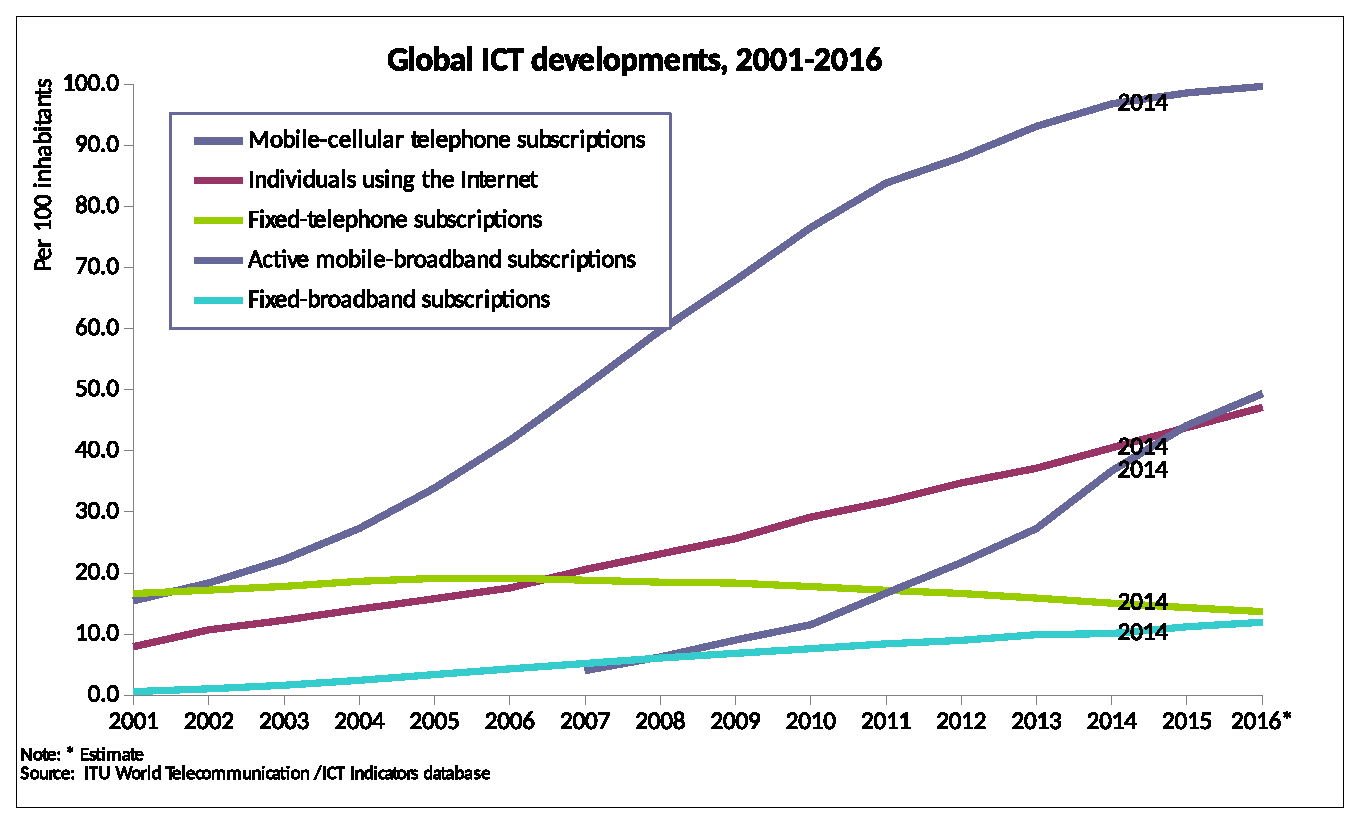
\includegraphics[width=1\textwidth]{images/ict_Developments-2001_2016} 

            \label{fig:ictAdoption}


        \end{figure}


    \end{frame}


    \begin{frame}{Introduction}{Where are we? Where are we heading?}

%        \begin{itemize}
%
%            \item<2> Desktop and laptop computers, smartphones and tablets, wearable devices, datacenters to support on-line services
%
%            \item<3> ``Internet of Things'' is coming
%
%
%        \end{itemize}

        \begin{figure}[h]

            \centering

$
            \begin{array}{ccc}

                \includegraphics[scale=0.125]{images/desktop} &
                \includegraphics[scale=0.25]{images/laptop} &
                \includegraphics[scale=0.25]{images/smartphone}
                \\
                \includegraphics[scale=0.25]{images/tablet} &
                \includegraphics[scale=0.25]{images/wearable} &
                \includegraphics[scale=0.25]{images/data_center}


            \end{array}
$

            \label{fig:devices}


        \end{figure}


    \end{frame}


    \begin{frame}{Introduction}{Where are we? Where are we heading?}

%        \begin{itemize}
%
%            \item<3> ``Internet of Things'' is coming
%
%
%        \end{itemize}

        \begin{figure}[h]

            \centering

$
            \begin{array}{ccc}

            \includegraphics[scale=0.25]{images/internet-of-things}
            \includegraphics[scale=0.375]{images/internet-of-things-adoption-prediction}

            \end{array}
$

            \label{fig:internetOfThings}

        \end{figure}

        \vfill
        \footnotesize{Source: http://cdn2.business2community.com/wp-content/uploads/2016/06/internet-of-things.jpg}


    \end{frame}


    %% %%%%%%%%%% %%%%%%%%%% %%%%%%%%%% %%%%%%%%%% %%%%%%%%%% %%%%%%%%%% %%%%%%%%%%

    %\begin{frame}{Introduction}{And it's not going to stop!}


    %\end{frame}


    %% %%%%%%%%%% %%%%%%%%%% %%%%%%%%%% %%%%%%%%%% %%%%%%%%%% %%%%%%%%%% %%%%%%%%%%

    \begin{frame}{Introduction}{And the problem is\ldots}

        %This increase in device usage leads to the increase of:

%        \begin{itemize}
%
%            \item<1> Energy consumption
%
%            \item<2> Greenhouse gases emission
%
%            \item<3> Monetary costs% (derived from the previous items)
%
%        \end{itemize}

        \begin{figure}[h]

            \centering

            %\includegraphics[width=.75\textwidth]{images/world_energy_consumption} 
            \includegraphics[width=.75\textwidth]{images/world-energy-consumption-for-each-fuel-2014-line} 

            \label{fig:worldEnergyConsumption}


        \end{figure}

        %\footnotesize{By Con-struct (BP Statistical Review of World Energy 2015) [GFDL (http://www.gnu.org/copyleft/fdl.html) or CC BY-SA 3.0 (http://creativecommons.org/licenses/by-sa/3.0)], via Wikimedia Commons}


        \footnotesize{Our Finite World blog by Gail Tverberg is licensed under a Creative Commons Attribution-ShareAlike 3.0 Unported License.}

    \end{frame}


    \begin{frame}{Introduction}{And the problem is\ldots}

        %This increase in device usage leads to the increase of:

%        \begin{itemize}
%
%            \item<2> Greenhouse gases emission
%
%            \item<3> Monetary costs% (derived from the previous items)
%
%        \end{itemize}

        \begin{figure}[h]

            \centering

$
            \begin{array}{cc}

            \includegraphics[width=.375\textwidth]{images/greenhouse-gas} &
            \includegraphics[width=.375\textwidth]{images/money-055}

            \end{array}
$

            \label{fig:greenhouseGasEmissionAndMoneyCosts}


        \end{figure}

        \footnotesize{DIBYANGSHU SARKAR/AFP/Getty Images}


    \end{frame}


%    \begin{frame}{Introduction}{And the problem is\ldots}
%
%        %This increase in device usage leads to the increase of:
%
%%        \begin{itemize}
%%
%%            \item<3> Monetary costs% (derived from the previous items)
%%
%%        \end{itemize}
%
%        \begin{figure}[h]
%
%            \centering
%
%            \includegraphics[width=.75\textwidth]{images/money-055} 
%
%            \label{fig:monetaryCosts}
%
%
%        \end{figure}
%
%
%    \end{frame}



    %% %%%%%%%%%% %%%%%%%%%% %%%%%%%%%% %%%%%%%%%% %%%%%%%%%% %%%%%%%%%% %%%%%%%%%%

    \begin{frame}{Introduction}{Some numbers\ldots}


        %The ICT sector alone, is responsible for:

%        \begin{itemize}
%
%            \item<1> 50\% of the energy costs of organizations
%
%            \item<2> 7\% of global energy consumption (expected to reach 14\% by 2020)
%
%
%        \end{itemize}

        %Enterprise energy costs

        \begin{figure}[h]

            \centering

$
            \begin{array}{cc}

            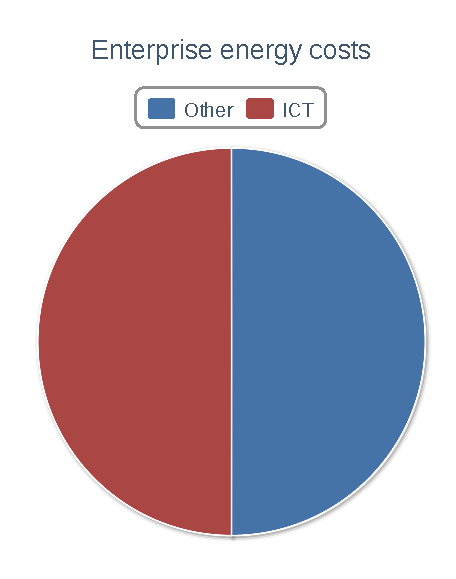
\includegraphics[width=.25\textwidth]{images/50-50} &
            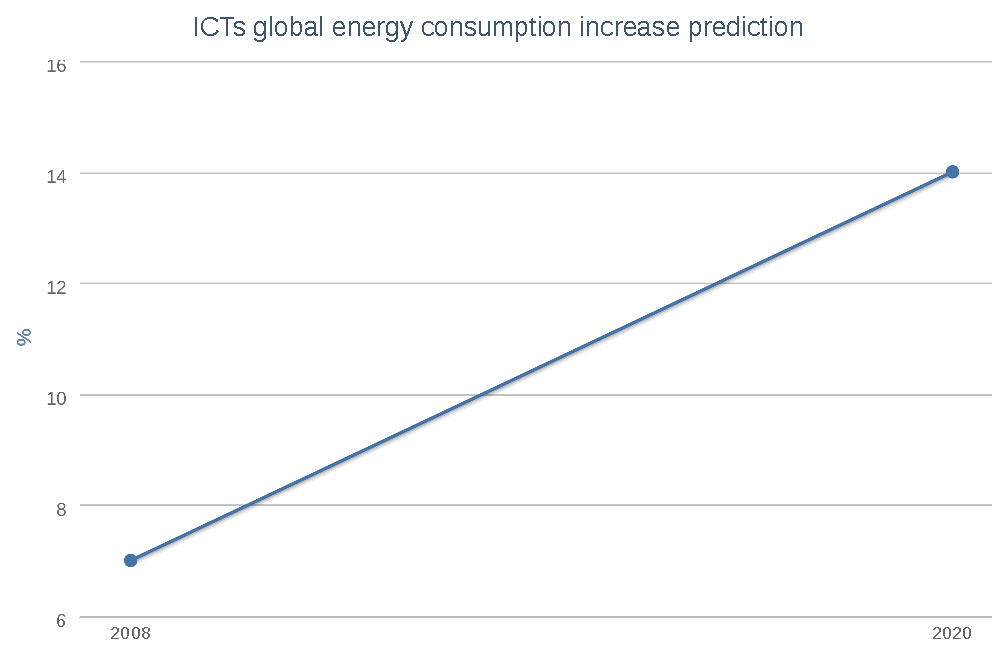
\includegraphics[width=.5\textwidth]{images/ictEnergyConsDoubleBy2020} 

            \end{array}
$

            \label{fig:entEnergyConsumption}


        \end{figure}


    \end{frame}


%    \begin{frame}{Introduction}{Some numbers\ldots}
%
%
%        %The ICT sector alone, is responsible for:
%
%%        \begin{itemize}
%%
%%            \item<2> 7\% of global energy consumption (expected to reach 14\% by 2020)
%%
%%
%%        \end{itemize}
%
%        ICTs global energy consumption increase prediction
%
%        \begin{figure}[h]
%
%            \centering
%
%            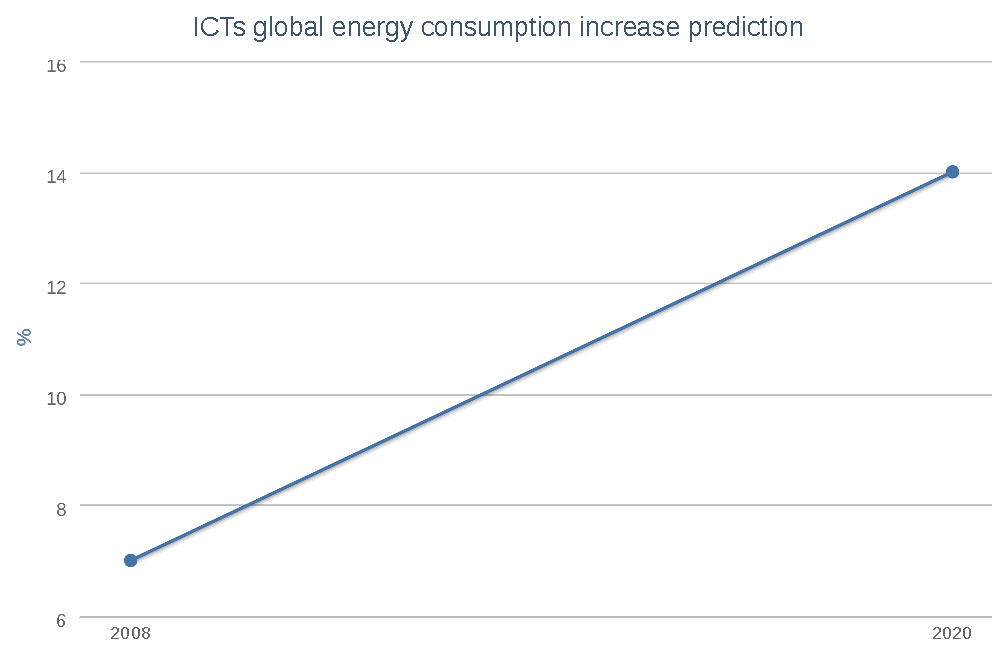
\includegraphics[width=.75\textwidth]{images/ictEnergyConsDoubleBy2020} 
%
%            \label{fig:ictEnergyConsDoubleBy2020}
%
%
%        \end{figure}
%
%
%    \end{frame}


    %% %%%%%%%%%% %%%%%%%%%% %%%%%%%%%% %%%%%%%%%% %%%%%%%%%% %%%%%%%%%% %%%%%%%%%%

    \begin{frame}{Introduction}{We must\ldots}

        %\begin{itemize}

            %\item ICTs help reduce energy/resource consumption in other, diverse, ``areas''


        %\end{itemize}
  
%        \begin{itemize}
%
%            \item Alleviate ICTs own energy footprint
%
%
%        \end{itemize}

        \begin{figure}[h]

            \centering

            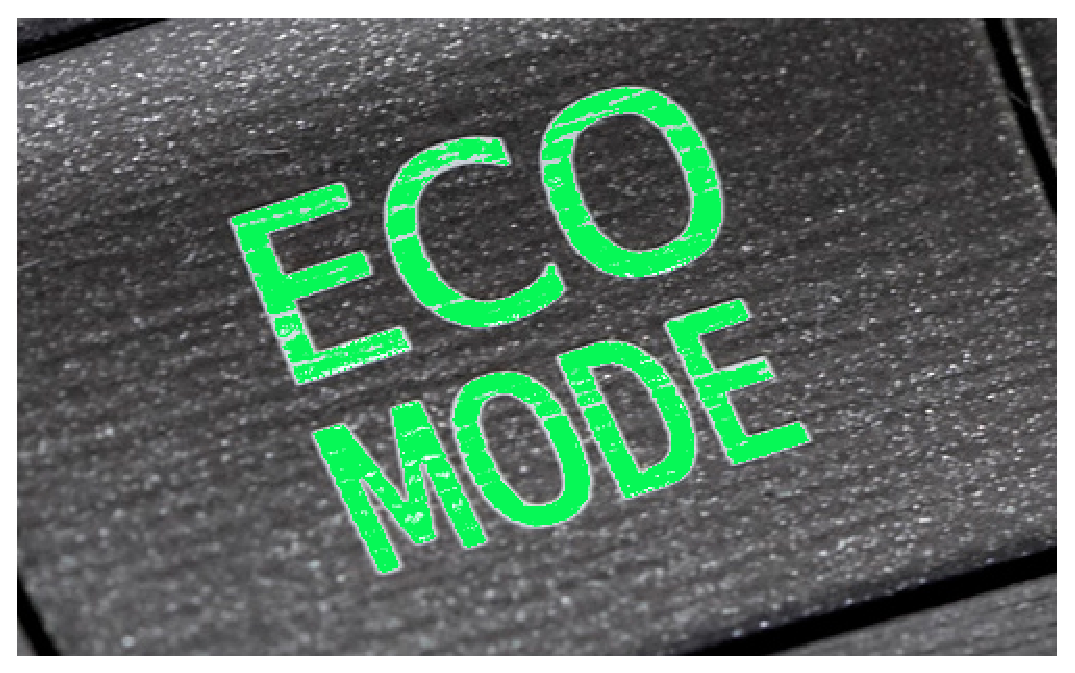
\includegraphics[width=.75\textwidth]{images/ecomode} 

            \label{fig:ecomode}


        \end{figure}


    \end{frame}


    %% %%%%%%%%%% %%%%%%%%%% %%%%%%%%%% %%%%%%%%%% %%%%%%%%%% %%%%%%%%%% %%%%%%%%%%

    \begin{frame}{Introduction}{We intend to\ldots}

        \begin{itemize}

            \item<1> Search possible gains in the energy consumption induced by software

            \begin{itemize}

                \item Maybe between 30\% and 90\%?

            \end{itemize}

            \item<2> Focus on the \Haskell language


        \end{itemize}

    \end{frame}


    %% %%%%%%%%%% %%%%%%%%%% %%%%%%%%%% %%%%%%%%%% %%%%%%%%%% %%%%%%%%%% %%%%%%%%%%

    \begin{frame}{Introduction}{We have\ldots}

        \begin{itemize}

            \item Investigated the \Edison library

            \begin{itemize}

                \item Refactoring, to use alternative data structure implementations

                \item Concerning Package and RAM energy consumptions

		\item Compiler optimizations effect


            \end{itemize}

            \item http://green-haskell.github.io


        \end{itemize}


    \end{frame}


    %% %%%%%%%%%% %%%%%%%%%% %%%%%%%%%% %%%%%%%%%% %%%%%%%%%% %%%%%%%%%% %%%%%%%%%%

    \begin{frame}{Introduction}{Research Question!}


        \RQ{}. How do execution time and Package and RAM energy consumptions are affected by the use of a lazy or strict data structure implementation?
        %\medskip
        %\pause


    \end{frame}


    %% %%%%%%%%%% %%%%%%%%%% %%%%%%%%%% %%%%%%%%%% %%%%%%%%%% %%%%%%%%%% %%%%%%%%%%


%% %%%%%%%%%% %%%%%%%%%% %%%%%%%%%% %%%%%%%%%% %%%%%%%%%% %%%%%%%%%% %%%%%%%%%%




        %% %%%%%%%%%% %%%%%%%%%% %%%%%%%%%% %%%%%%%%%% %%%%%%%%%% %%%%%%%%%% %%%%%%%%%%

\section{Approach}


    %% %%%%%%%%%% %%%%%%%%%% %%%%%%%%%% %%%%%%%%%% %%%%%%%%%% %%%%%%%%%% %%%%%%%%%%

    \begin{frame}[plain]{}

        \begin{center}

        \huge Approach

        \end{center}

    \end{frame}


    %% %%%%%%%%%% %%%%%%%%%% %%%%%%%%%% %%%%%%%%%% %%%%%%%%%% %%%%%%%%%% %%%%%%%%%%

    \begin{frame}{Data structures}{Maps}

        \begin{description}

            \item [Data.Map] a general-purpose implementation of ordered maps (dictionaries), based on balanced binary trees

            \item [Data.IntMap] an efficient implementation of maps, with integer keys, based on big-endian patricia trees

            \item [Data.HashMap] an implementation of unordered maps from hashable keys to values, optimized for performance, based on hash array mapped tries


        \end{description}


    \end{frame}


    %% %%%%%%%%%% %%%%%%%%%% %%%%%%%%%% %%%%%%%%%% %%%%%%%%%% %%%%%%%%%% %%%%%%%%%%

    \begin{frame}{Benchmark}{Benchmark Operations}

        \begin{table}[h]

            \centering

            %\caption{Benchmark Operations.}
            \label{tab:benchmarkOperations}

            \begin{tabular}{|c|c|c|c|}

                \hline

                $iters$ & $operation$ & $base$ & $elems$ \\
          
                \hline
                1     & add         & 100000 & 100000 \\
                1000  & addAll      & 100000 & 1000   \\
                1     & clear       & 100000 & n.a.   \\
                1000  & contains    & 100000 & 1      \\
                5000  & containsAll & 100000 & 1000   \\
                1     & iterator    & 100000 & n.a.   \\
                10000 & remove      & 100000 & 1      \\
                10    & removeAll   & 100000 & 1000   \\
                10    & retainAll   & 100000 & 1000   \\
                5000  & toArray     & 100000 & n.a.   \\
          
                \hline


            \end{tabular}


        \end{table}

	$$ iters * operation( base , elems ) $$

    \end{frame}


    %% %%%%%%%%%% %%%%%%%%%% %%%%%%%%%% %%%%%%%%%% %%%%%%%%%% %%%%%%%%%% %%%%%%%%%%

    \begin{frame}[fragile]{Benchmark}{Benchmark Operations}

	%\begin{lstlisting}[language=Haskell]
	\begin{verbatim}
removeAll :: Map Key Datum -> Map Key Datum -> Map Key Datum
removeAll = difference

retainAll :: Map Key Datum -> Map Key Datum -> Map Key Datum
retainAll = intersectionWith const
	\end{verbatim}
        %\end{lstlisting}


    \end{frame}


    %% %%%%%%%%%% %%%%%%%%%% %%%%%%%%%% %%%%%%%%%% %%%%%%%%%% %%%%%%%%%% %%%%%%%%%%

    \begin{frame}{An interface for measuring energy consumption}{RAPL}

        \begin{figure}[h]

            \centering

            %\caption{RAPL domains.}
            %\label{fig:raplDomains}

            \includegraphics[width=1\textwidth]{images/power_domains2.jpg}


        \end{figure}

        \footnotesize{Source: https://software.intel.com/en-us/articles/intel-power-governor}


    \end{frame}


    %% %%%%%%%%%% %%%%%%%%%% %%%%%%%%%% %%%%%%%%%% %%%%%%%%%% %%%%%%%%%% %%%%%%%%%%

    \begin{frame}[fragile]{Benchmark execution and analysis}{Criterion}

        \begin{verbatim}
import Criterion.Main

-- Our benchmark harness.
main = defaultMain [
    bgroup "Map/" [
        env (...) -> bench addAllOpDesc $
            nf ( addAllNTimes a b ) addAllNRepeats
    ]
]
        \end{verbatim}


    \end{frame}


    %% %%%%%%%%%% %%%%%%%%%% %%%%%%%%%% %%%%%%%%%% %%%%%%%%%% %%%%%%%%%% %%%%%%%%%%

    \begin{frame}[fragile]{Benchmark execution and analysis}{Criterion}

        \begin{verbatim}
benchmarking (...)/addAll_1000_times_1000_elements_to_100000
time                 1.245 s    (1.234 s .. 1.261 s)
                     1.000 R^2   (1.000 R^2 .. 1.000 R^2)
mean                 1.248 s    (1.246 s .. 1.251 s)
std dev              3.883 ms   (0.0 s .. 4.130 ms)
packageEnergy:       1.000 R^2   (0.998 R^2 .. 1.000 R^2)
  iters              31.288     (29.594 .. 33.275)
  y                  0.545      (-2.154 .. 5.209)
dramEnergy:          1.000 R^2   (1.000 R^2 .. 1.000 R^2)
  iters              10.404     (10.214 .. 10.680)
  y                  0.121      (-0.262 .. 0.671)
        \end{verbatim}


    \end{frame}


    %% %%%%%%%%%% %%%%%%%%%% %%%%%%%%%% %%%%%%%%%% %%%%%%%%%% %%%%%%%%%% %%%%%%%%%%


%% %%%%%%%%%% %%%%%%%%%% %%%%%%%%%% %%%%%%%%%% %%%%%%%%%% %%%%%%%%%% %%%%%%%%%%




        %% %%%%%%%%%% %%%%%%%%%% %%%%%%%%%% %%%%%%%%%% %%%%%%%%%% %%%%%%%%%% %%%%%%%%%%

\section{Results}


    %% %%%%%%%%%% %%%%%%%%%% %%%%%%%%%% %%%%%%%%%% %%%%%%%%%% %%%%%%%%%% %%%%%%%%%%

    \begin{frame}[plain]{}

        \begin{center}

        \huge Results

        \end{center}

    \end{frame}

    %% %%%%%%%%%% %%%%%%%%%% %%%%%%%%%% %%%%%%%%%% %%%%%%%%%% %%%%%%%%%% %%%%%%%%%%

    \begin{frame}{Results}{Lazy vs Strict, Iterator}

        \begin{figure}[h]

            \centering

$
            \begin{array}{cc}

                \includegraphics[scale=0.3125]{images/bench_Results/plot_iterator_100000_elements_time} &
                \includegraphics[scale=0.3125]{images/bench_Results/plot_iterator_100000_elements_energy_package}
                \\
		\multicolumn{2}{c}{\includegraphics[scale=0.3125]{images/bench_Results/plot_iterator_100000_elements_energy_dram}}


            \end{array}
$

            \label{fig:resultsValues}


        \end{figure}


    \end{frame}


    %% %%%%%%%%%% %%%%%%%%%% %%%%%%%%%% %%%%%%%%%% %%%%%%%%%% %%%%%%%%%% %%%%%%%%%%

    \begin{frame}{Results}{}

        \begin{figure}[h]

            \centering

$
            \begin{array}{cc}

                \includegraphics[scale=0.3125]{images/bench_Results/map_differences} &
                \includegraphics[scale=0.3125]{images/bench_Results/intmap_differences}
                \\
		\multicolumn{2}{c}{\includegraphics[scale=0.3125]{images/bench_Results/hashmap_differences}}


            \end{array}
$

            \label{fig:resultsImprovementsStrictOverLazy}


        \end{figure}


    \end{frame}


    %% %%%%%%%%%% %%%%%%%%%% %%%%%%%%%% %%%%%%%%%% %%%%%%%%%% %%%%%%%%%% %%%%%%%%%%


    %% %%%%%%%%%% %%%%%%%%%% %%%%%%%%%% %%%%%%%%%% %%%%%%%%%% %%%%%%%%%% %%%%%%%%%%


    %% %%%%%%%%%% %%%%%%%%%% %%%%%%%%%% %%%%%%%%%% %%%%%%%%%% %%%%%%%%%% %%%%%%%%%%


%% %%%%%%%%%% %%%%%%%%%% %%%%%%%%%% %%%%%%%%%% %%%%%%%%%% %%%%%%%%%% %%%%%%%%%%




        %% %%%%%%%%%% %%%%%%%%%% %%%%%%%%%% %%%%%%%%%% %%%%%%%%%% %%%%%%%%%% %%%%%%%%%%

\section{Conclusions}


    %% %%%%%%%%%% %%%%%%%%%% %%%%%%%%%% %%%%%%%%%% %%%%%%%%%% %%%%%%%%%% %%%%%%%%%%

    \begin{frame}[plain]{}

        \begin{center}

		\huge Conclusions

        \end{center}

    \end{frame}


    %% %%%%%%%%%% %%%%%%%%%% %%%%%%%%%% %%%%%%%%%% %%%%%%%%%% %%%%%%%%%% %%%%%%%%%%

    \begin{frame}{Conclusions}{The answer to the RQ. is...}

        \RQ{}. How do execution time and Package and RAM energy consumptions are affected by the use of a lazy or strict data structure implementation?

        \medskip

        \begin{itemize}

            \item Energy consumption is proportional to the execution time, and
	    \item strict evaluation tends to be more efficient in terms of execution time and energy consumption than the lazy evaluation


        \end{itemize}


    \end{frame}


    %% %%%%%%%%%% %%%%%%%%%% %%%%%%%%%% %%%%%%%%%% %%%%%%%%%% %%%%%%%%%% %%%%%%%%%%

    \begin{frame}[plain]{}

        \begin{center}

		\huge Future Work

        \end{center}

    \end{frame}


    %% %%%%%%%%%% %%%%%%%%%% %%%%%%%%%% %%%%%%%%%% %%%%%%%%%% %%%%%%%%%% %%%%%%%%%%


    \begin{frame}{Future Work}{What's next?}

        \begin{itemize}

            \item create/use more real-world benchmarks
            \item explore laziness vs strictness in more complex algorithms that rely on data structures (sorting or graph search algorithms)


        \end{itemize}


    \end{frame}


    %% %%%%%%%%%% %%%%%%%%%% %%%%%%%%%% %%%%%%%%%% %%%%%%%%%% %%%%%%%%%% %%%%%%%%%%


%% %%%%%%%%%% %%%%%%%%%% %%%%%%%%%% %%%%%%%%%% %%%%%%%%%% %%%%%%%%%% %%%%%%%%%%





        %% %%%%%%%%%% %%%%%%%%%% %%%%%%%%%% %%%%%%%%%% %%%%%%%%%% %%%%%%%%%% %%%%%%%%%%

        \begin{frame}

            \maketitle

            \includegraphics[width=.25\textwidth]{images/i_m_saving_energy} 


        \end{frame}


        %% %%%%%%%%%% %%%%%%%%%% %%%%%%%%%% %%%%%%%%%% %%%%%%%%%% %%%%%%%%%% %%%%%%%%%%


    \end{document}


%% %%%%%%%%%% %%%%%%%%%% %%%%%%%%%% %%%%%%%%%% %%%%%%%%%% %%%%%%%%%% %%%%%%%%%%


